% -*- root: ../../../main.tex -*-
\subsection{Safety e Consistency}
Nelle sezioni precedenti è stato descritto il funzionamento principale di \textbf{RAFT}, tralasciando alcune proprietà e vincoli essenziali per mantenere consistenza tra i log.
Attualmente ci sono casi che non sono gestiti, casi che possono causare noitevole inconsistenza tra i log.
Questa proprietà serve per prevenire che due o più macchine eseguano una sequenza diversa di comandi causando inconsistenza.
Ad esempio se il \textbf{Leader} \textit{valida} alcune \textit{entry} mentre un dato \textbf{Follower} è offline; se successivamente il \textbf{Follower} viene eletto sovrascriverà le entry gia eseguite, e ne eseguirà altre.  
\\
Di seguito riportiamo tutte le proprietà che \textbf{RAFT} mette in campo per evitare che un caso del genere si verifichi:
\begin{enumerate}
	\item Election Safety: Per un dato term è possibile al più eleggere un solo \textbf{Leader}.
	Il protocollo \textbf{RAFT} è modellato in maniera concentrica in un solo \textbf{Leader}, è quindi ovviamente necessaria questa proprietà.
	La dimostrazione di questa proprietà è già stata discussa precedentemente nella sezione \ref{electionsaf} alla pagina \pageref{electionsaf}.
	\item Leader Append-Only:Il \textbf{Leader} non cancella mai, ne sovrascrive le entry del proprio log(può sovrascrivere le entry dei \textbf{Follower}).

	\item Log Matching:Se due log contengono un \textit{entry} con lo stesso \textit{index} e stesso \textit{term}, allora le due \textit{entry} sono identiche e contengono la stessa sequenza di comandi, questo vale anche per tutte le \textit{entry} precedenti.
	Questa proprietà è costituita da due sottoproprietà:
	\begin{enumerate}
		\item Se due log hanno un entry con lo stesso index e stesso term, allora quell'entry contiene lo stesso comando(sono identiche).
		\item Se due \textit{entry} in log diversi hanno lo stesso index e lo stesso term, allora anche tutte le loro precedenti entry sono identiche tra i due log.
	\end{enumerate}
	La prima sottoproprietà deriva dal fatto che il \textbf{Leader} per un dato term assegnerà ad un dato indice al più una sola \textit{entry}.
	Mentre la seconda è garantità da un controllo effettuato dal \textbf{Follower} nel momento in cui verifica le \textit{entry} ricevute dal \textbf{Leader}.
	Questo meccanismo è spiegato in dettaglio nella sezione \ref{Log Replication} e nelle figure  \ref{fig:figure6} e \ref{fig:figure7}
	\item Leader Completeness:Se una \textit{entry} è validata(effettua il commit) in un certo term, allora tutti i \textbf{Leader} dei \textit{term} futuri avranno presente questa entry nel loro log.
	\item State Machine Safety:Se un qualunque \textbf{Server} esegue un \textit{entry} ad un certo index, allora nessun altro \textbf{Server} eseguirà un comando diverso allo stesso \textit{index}.
\end{enumerate}
  \subsubsection{Election restriction}
  	Durante le elezioni ci sono casi in cui non è possibile determinare se un \textit{entry} è validata oppure no.
  	In figura \ref{fig:figure 8} non è possibile determinare in quello scenario se l'ultima \textit{entry} è stata validata, per questo si aggiunge un ulteriore vincolo all'elezione di un \textbf{Candidate}.
  	Si restringere il range di elezione ai \textbf{Candidate} con il log più completo; questo per eleggere in ogni \textit{term} il migior \textbf{Candidate} quello che ha la visione più completa della situazione. 
  	Come già detto un candidate invia ad ogni elezione le informazioni riguardanti il log.
  	Più precisamente il \textbf{Candidate} invia solo le informazioni sull'ultima entry, l'\textit{index} e il \textit{term}, dato che queste informazioni definisco interamente il \textit{log}.
  	\\
  	Il criterio con cui viene fatta questa valutazione è il seguente: se l'ultimo term del log di V (votante) è maggiore di quello del log di C (candidato), allora la  richiesta viene rifiutata. Se invece i due ultimi term si equivalgono, la valutazione viene fatta tenendo conto della lunghezza del log. Se l'ultimo indice del log di C è maggiore di quello di V la richiesta viene accettata, altrimenti viene rifiutata.
  	
  \begin{figure}[H]
  	\centering
  	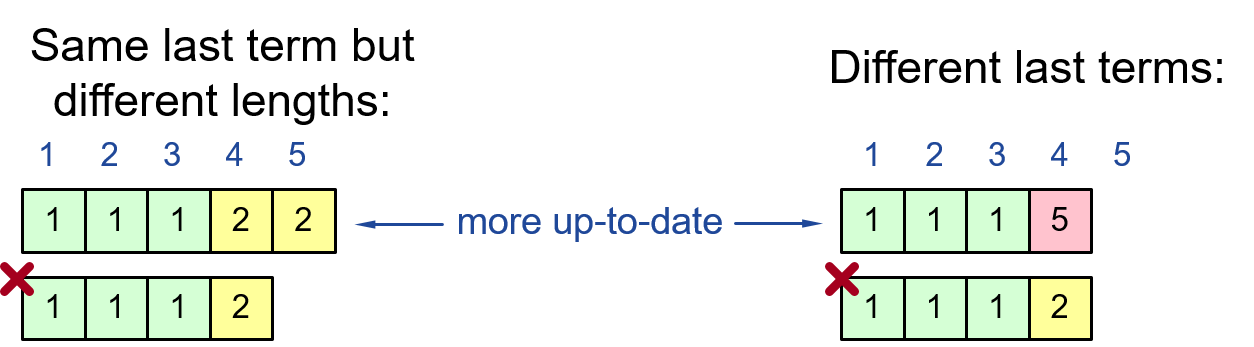
\includegraphics[width=0.99\columnwidth]{raft/pickingUpToDateLeader}
  	\captionsetup{singlelinecheck=off}
  	\caption[stateDiagramCaption]{
	In questo caso non è possibile determinare se l'ultima \textit{entry} è validata, inoltre solo il primo server può essere eletto dato che il terzo non è disponibile.}
  	\label{fig:figure8}
  \end{figure}
  \subsubsection{Committing entries from previous terms}
  \subsubsection{Neutralize Old Leaders}
  \subsubsection{Follower and Candidate Crash}
  \subsubsection{Timing and Availability}